\documentclass[tikz, border=3mm]{standalone}
\usepackage{tikz}
\usetikzlibrary{calc} % calc library for midpoints and fractional positions

\begin{document}
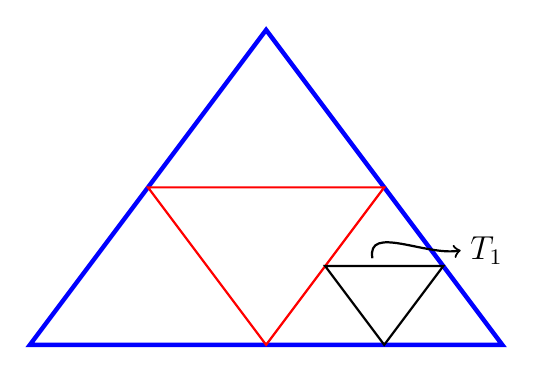
\begin{tikzpicture}

    % Define Outer Triangle Vertices
    \coordinate (A) at (-3, 0);
    \coordinate (B) at (3, 0);
    \coordinate (C) at (0, 4);

    % Calculate Red Triangle Vertices (midpoints of outer sides)
    \coordinate (D) at ($(A)!0.5!(B)$); % Midpoint of AB -> (0, 0)
    \coordinate (E) at ($(B)!0.5!(C)$); % Midpoint of BC -> (1.5, 2)
    \coordinate (F) at ($(C)!0.5!(A)$); % Midpoint of CA -> (-1.5, 2)

    % Calculate Black Triangle Vertices based on your description
    % Vertex 1: 0.25 along side BA (from B towards A)
    \coordinate (P1) at ($(B)!0.25!(A)$); % (1.5, 0)
    % Vertex 2: 0.25 along side BC (from B towards C)
    \coordinate (P2) at ($(B)!0.25!(C)$); % (2.25, 1)
    % Vertex 3: Midpoint of side FE of the RED triangle
    \coordinate (P3) at ($(D)!0.5!(E)$); % (0, 2)

    % Draw Triangles
    % 1. Big Blue Triangle
    \draw[blue, ultra thick] (A) -- (B) -- (C) -- cycle;

    % 2. Red Triangle (Midpoints)
    \draw[red, thick] (D) -- (E) -- (F) -- cycle;

    % 3. Black Triangle (Constructed as specified)
    \draw[black, thick] (P1) -- (P2) -- (P3) -- cycle;
    
    
     % --- Add Label T1 and Arrow ---
    % Position the label node first
    \node[font=\large] (T1label) at (2.8, 1.2) {$T_1$};
    % Draw a curved arrow pointing from near the black triangle vertex P2 to the label
    \draw[->, thick] ($(P3)+(0.6,0.1)$) to[out=100, in=190] (T1label.west);
    % --- End Label and Arrow ---

\end{tikzpicture}
\end{document}